%%%%%%%%%%%%%%
%% main.tex %%
%%%%%%%%%%%%%%

%% goal: latex script to assemble results of supporting/scripts into a main pdf figure file

%% author: Willem Bonnaffe (w.bonnaffe@gmail.com)

%% update log:

%%%%%%%%%%%%%%
%% INITIATE %%
%%%%%%%%%%%%%%

%% setup
\documentclass[multi=page]{standalone}
%
%% tikzipicture
\usepackage{tikz}
%
% %% to use sans serif font
% \renewcommand{\familydefault}{\sfdefault}
% \usepackage{helvet}
\usepackage{mathptmx} % (times)

\begin{document}

%%%%%%%%%%%%%%
%% COMMANDS %%
%%%%%%%%%%%%%%

%% figurePage
%% goal: create a new figure page
% @arg1 - scaling of content of figure page
% @arg2 - content of figure page
\newcommand{\figurePage}[2]{
	\begin{page}
		\begin{tikzpicture}
			\node [minimum size = 18cm,rectangle,fill=white] at (0,0) {}; %% frame
			\node [scale=#1] at (0,0) {
				#2
			};
		\end{tikzpicture}
	\end{page}
}

%% cropMask
%% goal: create a crop mask function
% @arg1 - width of mask
% @arg2 - height of mask
% @arg3 - x center of mask content
% @arg4 - y center of mask content
% @arg5 - x position of mask 
% @arg6 - y position of mask
% @arg7 - content of mask
\newcommand{\cropMask}[7]{
	\node [minimum width=#1,minimum height=#2,path picture={
			\node at (#3,#4) {
				#7
			};
		}] at (#5,#6) {};
}

%
%%%

%%%%%%%%%%%%%%%%%%%%%%%%%%%
%% SUPPLEMENTARY FIGURES %%
%%%%%%%%%%%%%%%%%%%%%%%%%%%

%% FIGURE S
\figurePage{.9}{
	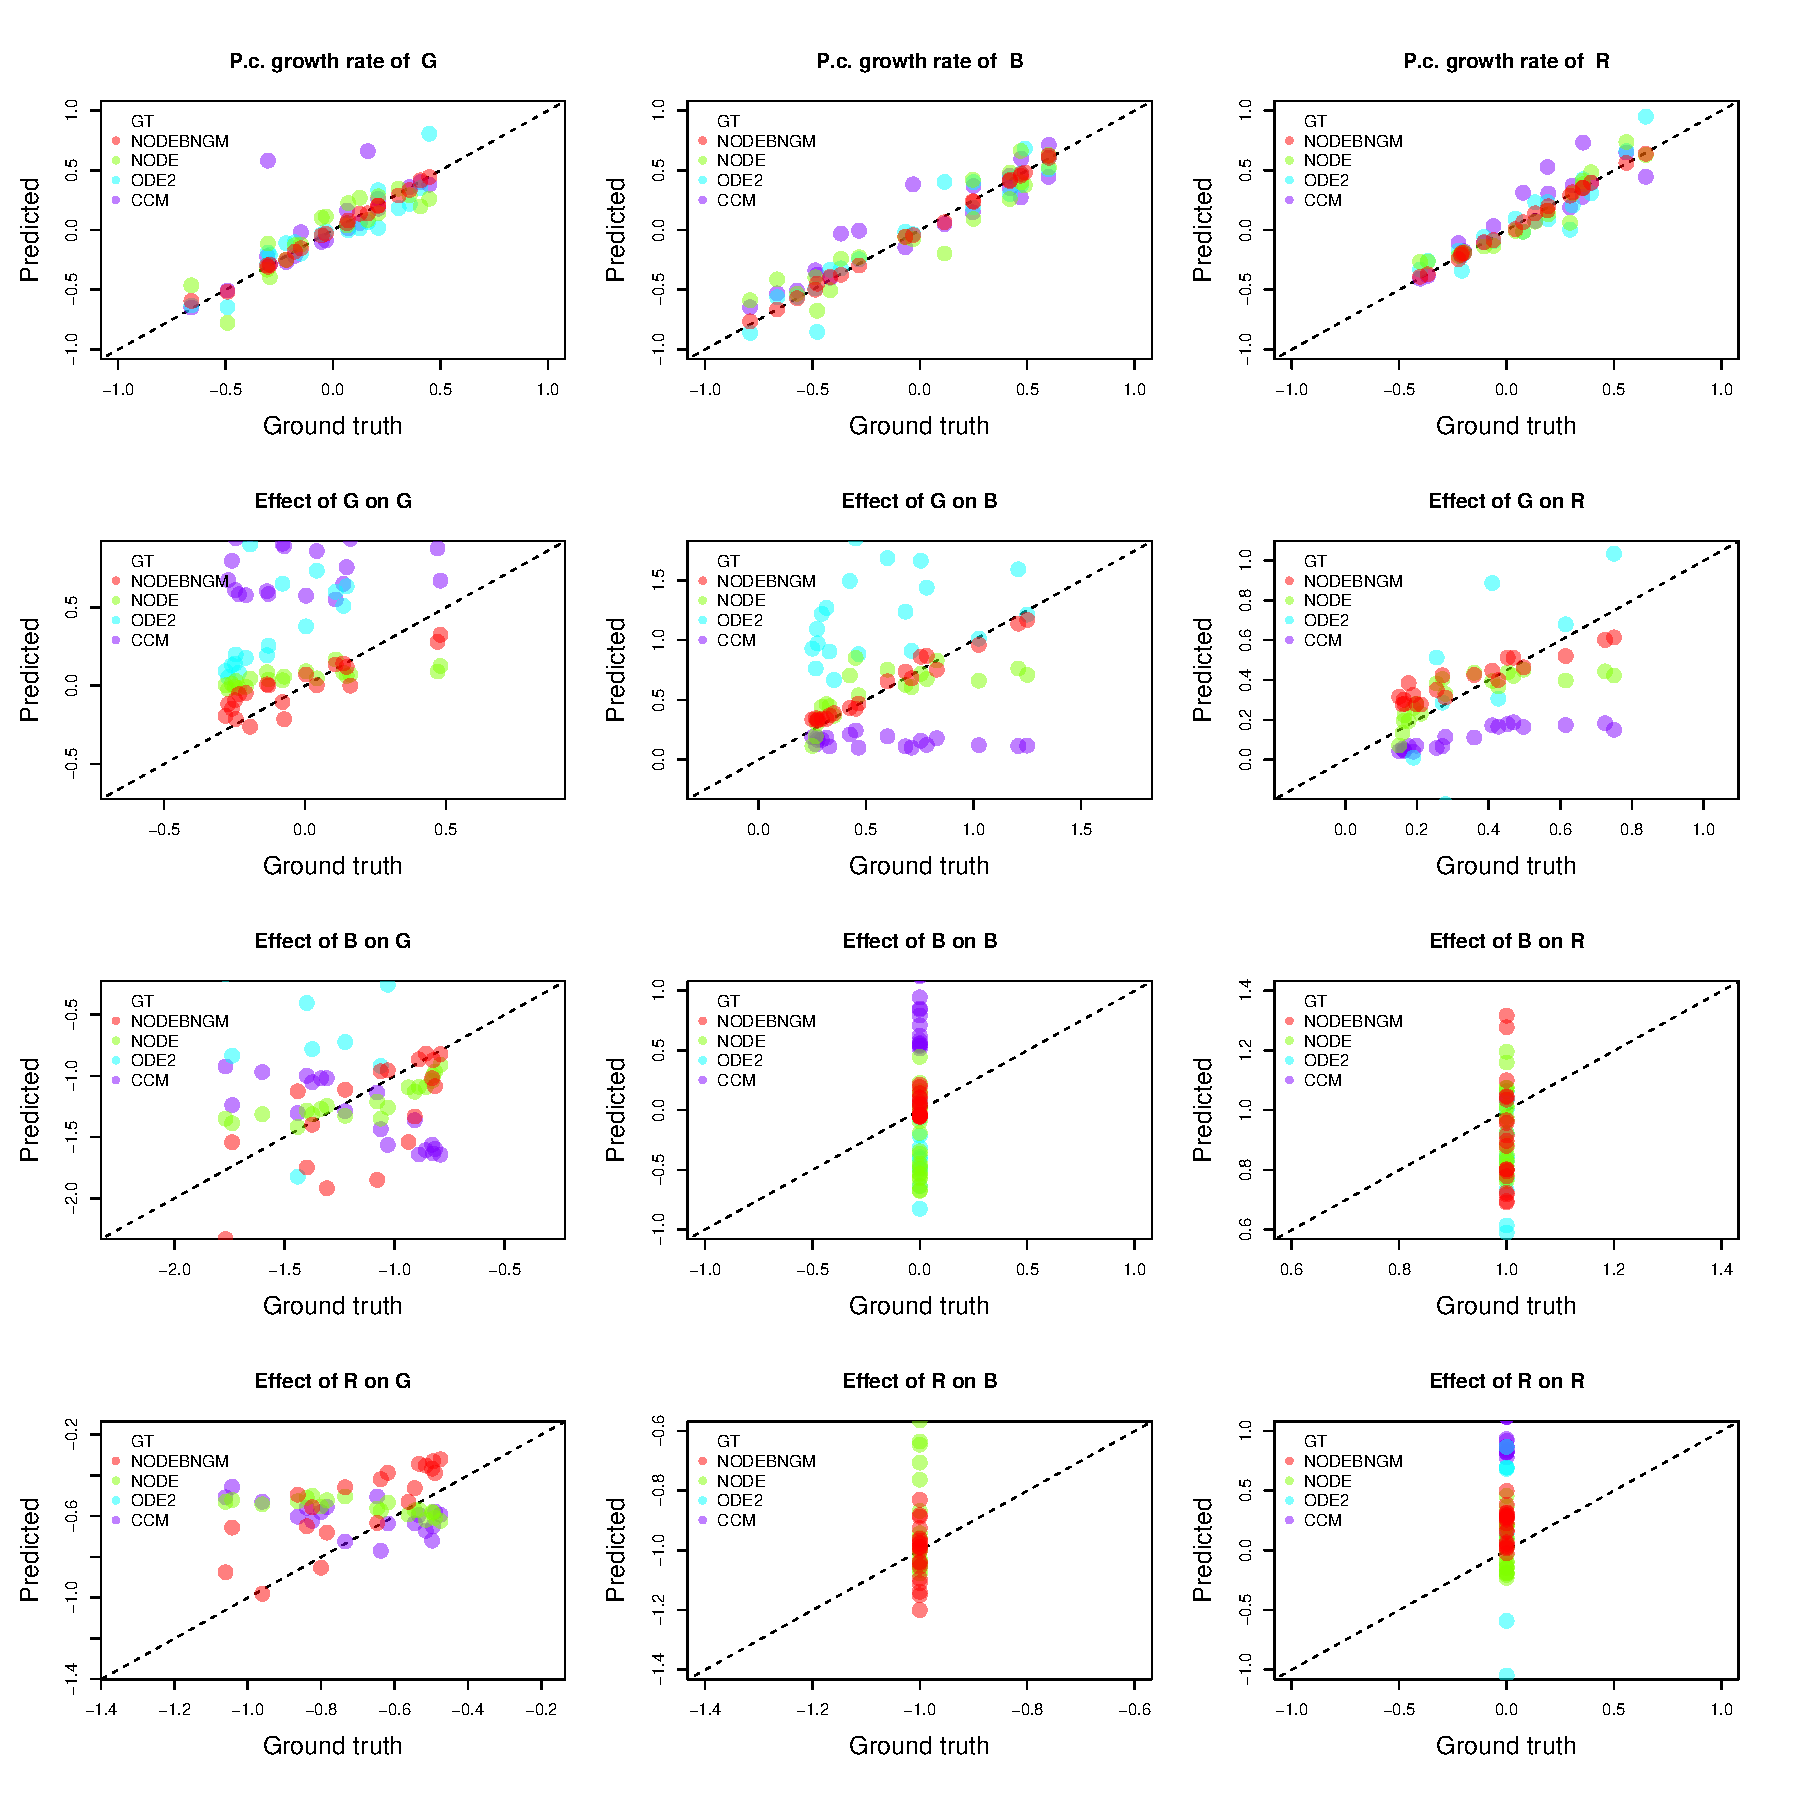
\includegraphics[page=1,width=18cm]{"supporting/scripts/benchmark/out/benchmark_train.pdf"}
}

%% FIGURE S
\figurePage{.9}{
	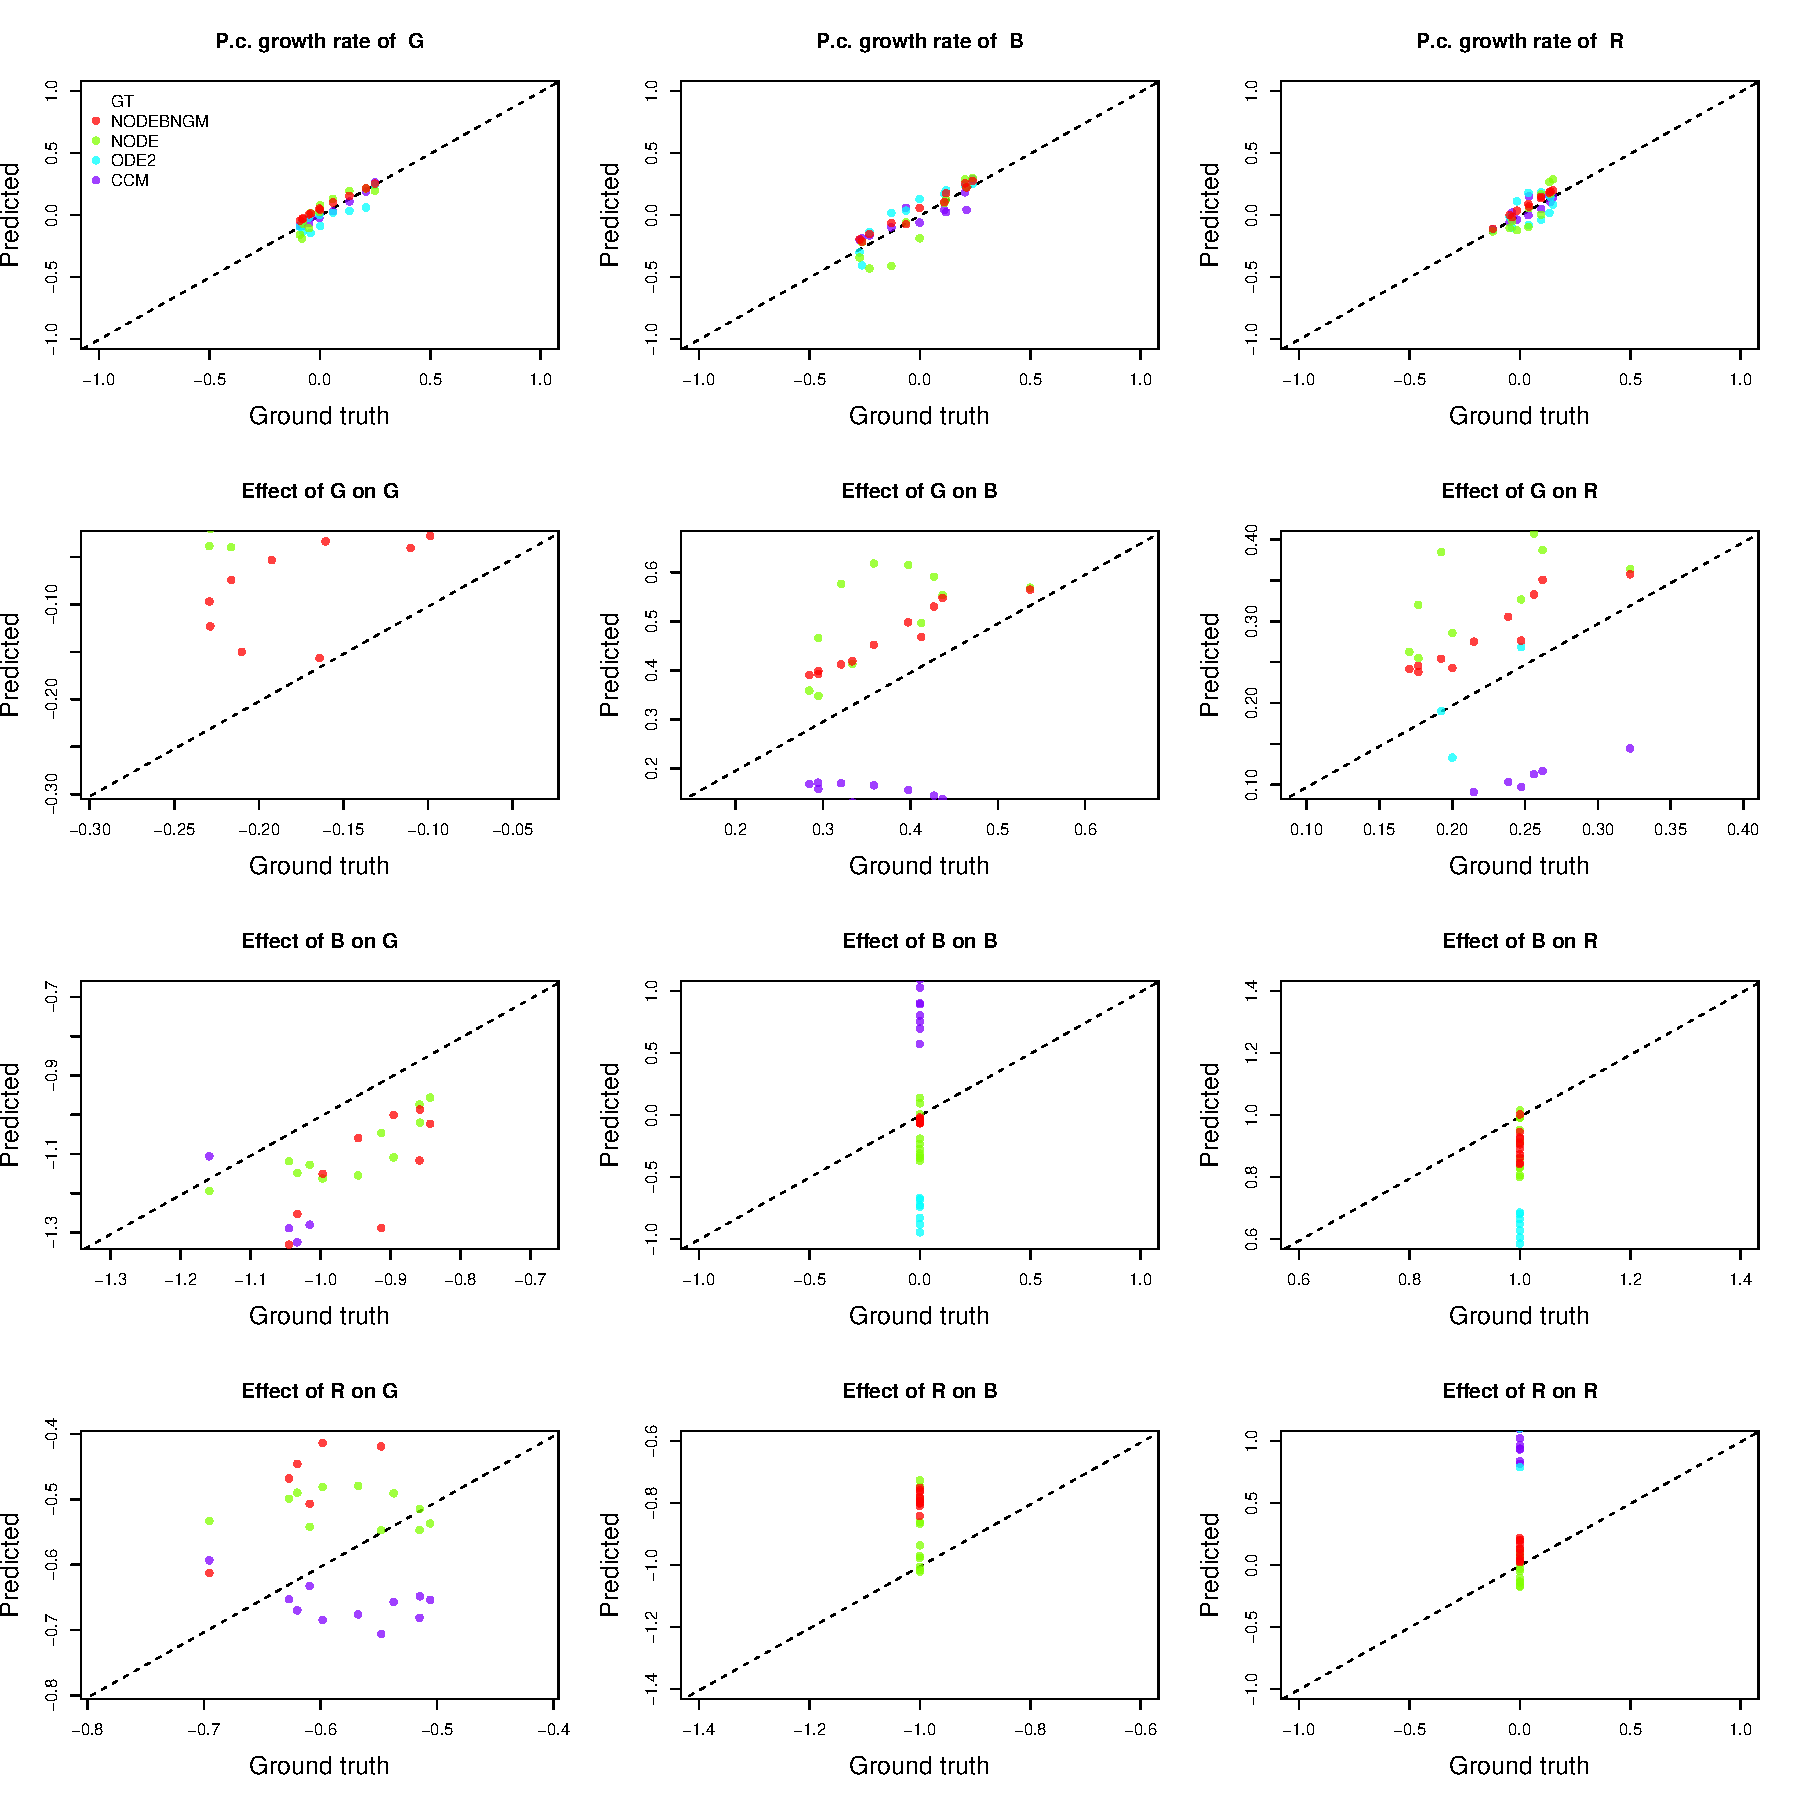
\includegraphics[page=1,width=18cm]{"supporting/scripts/benchmark/out/benchmark_test.pdf"}
}

%% FIGURE S
\figurePage{.9}{
	\includegraphics[page=1,width=18cm]{"supporting/scripts/benchmark/NODE/out/effects.pdf"}
}

%% FIGURE S
\figurePage{.9}{
	\includegraphics[page=1,width=18cm]{"supporting/scripts/benchmark/ODE2/out/effects.pdf"}
}
%% FIGURE S
\figurePage{.9}{
	\includegraphics[page=1,width=18cm]{"supporting/scripts/benchmark/CCM/out/effects.pdf"}
}

%% FIGURE S
\figurePage{.9}{
	\includegraphics[page=1,width=18cm]{"supporting/scripts/cmdline_TS1/out/fig_predictions_o.pdf"}
}

%% FIGURE S
\figurePage{.9}{
	\includegraphics[page=1,width=18cm]{"supporting/scripts/cmdline_TS1/out/fig_crossVal_p.pdf"}
}

%% FIGURE S
\figurePage{.9}{
	\includegraphics[page=1,width=18cm]{"supporting/scripts/cmdline_TS1/out/fig_predictions_p.pdf"}
}

%% FIGURE S
\figurePage{.9}{
	\includegraphics[page=1,width=18cm]{"supporting/scripts/cmdline_TS2/out/fig_predictions_o.pdf"}
}

%% FIGURE S
\figurePage{.9}{
	\includegraphics[page=1,width=18cm]{"supporting/scripts/cmdline_TS2/out/fig_crossVal_p.pdf"}
}

%% FIGURE S
\figurePage{.9}{
	\includegraphics[page=1,width=18cm]{"supporting/scripts/cmdline_TS2/out/fig_predictions_p.pdf"}
}

%% FIGURE S
\figurePage{.9}{
	\includegraphics[page=1,width=18cm]{"supporting/scripts/cmdline_TS3/out/fig_predictions_o.pdf"}
}

%% FIGURE S
\figurePage{.9}{
	\includegraphics[page=1,width=18cm]{"supporting/scripts/cmdline_TS3/out/fig_crossVal_p.pdf"}
}

%% FIGURE S
\figurePage{.9}{
	\includegraphics[page=1,width=18cm]{"supporting/scripts/cmdline_TS3/out/fig_predictions_p.pdf"}
}

%% FIGURE S
\figurePage{.9}{
	\includegraphics[page=1,width=18cm]{"supporting/scripts/cmdline_HL/out/fig_predictions_o.pdf"}
}

%% FIGURE S
\figurePage{.9}{
	\includegraphics[page=1,width=18cm]{"supporting/scripts/cmdline_HL/out/fig_crossVal_p.pdf"}
}

%% FIGURE S
\figurePage{.9}{
	\includegraphics[page=1,width=18cm]{"supporting/scripts/cmdline_HL/out/fig_predictions_p.pdf"}
}

%% FIGURE S
\figurePage{.9}{
	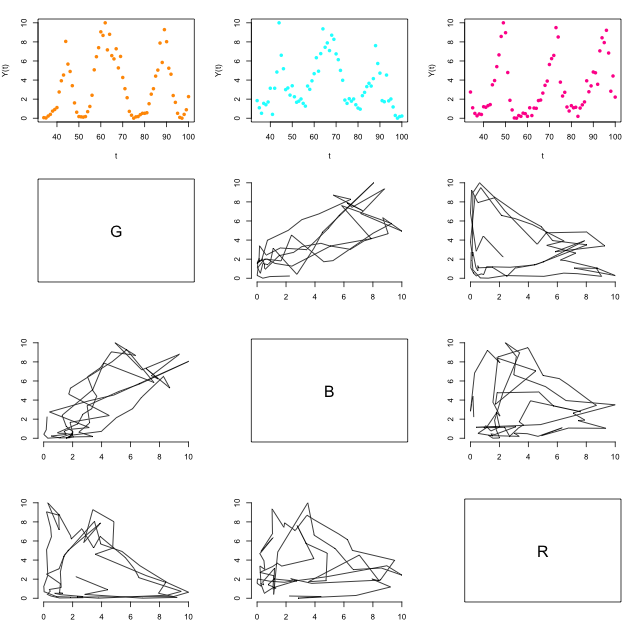
\includegraphics[page=1,width=18cm]{"supporting/scripts/RStudio_Ushio/out/fig_time_series.pdf"}
}

%% FIGURE S
\figurePage{.9}{
	\includegraphics[page=1,width=18cm]{"supporting/scripts/RStudio_Ushio/out/fig_predictions_o.pdf"}
}

%% FIGURE S
\figurePage{.9}{
	\includegraphics[page=2,width=18cm]{"supporting/scripts/RStudio_Ushio/out/fig_predictions_o.pdf"}
}

%% FIGURE S
\figurePage{.9}{
	\includegraphics[page=3,width=18cm]{"supporting/scripts/RStudio_Ushio/out/fig_predictions_o.pdf"}
}

%% FIGURE S
\figurePage{.9}{
	\includegraphics[page=4,width=18cm]{"supporting/scripts/RStudio_Ushio/out/fig_predictions_o.pdf"}
}

%% FIGURE S
\figurePage{.9}{
	\includegraphics[page=1,width=18cm]{"supporting/scripts/RStudio_Ushio/out/fig_crossVal_p.pdf"}
}

%% FIGURE S
\figurePage{.9}{
	\includegraphics[page=2,width=18cm]{"supporting/scripts/RStudio_Ushio/out/fig_crossVal_p.pdf"}
}

%% FIGURE S
\figurePage{.9}{
	\includegraphics[page=3,width=18cm]{"supporting/scripts/RStudio_Ushio/out/fig_crossVal_p.pdf"}
}

%% FIGURE S
\figurePage{.9}{
	\includegraphics[page=4,width=18cm]{"supporting/scripts/RStudio_Ushio/out/fig_crossVal_p.pdf"}
}

%% FIGURE S
\figurePage{.9}{
	\includegraphics[page=1,width=18cm]{"supporting/scripts/RStudio_Ushio/out/fig_predictions_p.pdf"}
}

%% FIGURE S
\figurePage{.9}{
	\includegraphics[page=2,width=18cm]{"supporting/scripts/RStudio_Ushio/out/fig_predictions_p.pdf"}
}

%% FIGURE S
\figurePage{.9}{
	\includegraphics[page=3,width=18cm]{"supporting/scripts/RStudio_Ushio/out/fig_predictions_p.pdf"}
}

%% FIGURE S
\figurePage{.9}{
	\includegraphics[page=4,width=18cm]{"supporting/scripts/RStudio_Ushio/out/fig_predictions_p.pdf"}
}

%
%%%

\end{document}
